%%%%%%%%%%%%%%%%%%%%
%% KAPITEL Server %%
%%%%%%%%%%%%%%%%%%%%
%% STEFFEN
%%%%%%%%%%%%%%%%%%%%%
% kurze Grundlage, dass man Server braucht (sowohl Applikationsserver -> für ERP,...; als auch Storageserver, wo Daten abgelegt werden (!=App. Server => Redudanz), als auch welche Betriebssysteme von SAP grundsätzlich unterstützt werden
Die technologische Architektur beschreibt die Technologien, die genutzt werden, um Geschäftsprozesse zu unterstützen. Sie beschreibt also Hardware, Betriebssysteme, Datenbanken und applikationsspezifische Technologien, die zusammenkommen müssen, um eine Grundlage für eine betrieblich genutzte Applikation zu bilden.\\
Wenn diese eine \gls{sap}-Applikation ist, wird diese Kombination als "`\gls{sap} Basis"' bezeichnet.
Eine Grundlage hier bildet gut aufeinander abgestimmte Hardware für \gls{sap} Systeme. Dabei bestehen diese Systeme aus Servern, Plattenspeicher-Systemen und Netzwerkausrüstung, wie \gls{zb} Routern, Switches oder Firewalls. Die benötigten Komponenten können entweder selbst in einem eigenen Rechenzentrum betrieben werden, ausgelagert \gls{bzw} in \gls{iaas} Umgebungen betrieben werden.\\
Diese Systeme sind mit einem Betriebssystem bespielt, welches wir für unsere Zwecke als Software bezeichnen, die es einer Anwendung wie einer \gls{db} oder \gls{sap} erlaubt auf die Ressourcen der Hardware zuzugreifen. Es dient also als Vermittler zwischen Hard- und Software.
In heutigen \gls{sap} Umgebungen sind Betriebssysteme wie \emph{Microsoft Windows Server}, \emph{Red Hat Enterprise Linux}, \emph{SuSE Linux}, sowie verschiedene \emph{UNIX} Derivate geläufig. Auch Host-Betriebssysteme (\emph{z/OS}, \emph{OS400}) werden als Plattform eines \gls{sap}-Systems unterstützt \cite{SAPin24hrs}. 

\section{SAP GUI}
\label{sec:sapgui}

\section{SAP NetWeaver Plattform}
\label{sec:netweaver}
In einer Ergänzung im Zuge einer Aktualisierung der Basisarchitektur wurden dem \gls{sap} Web Application Server ca. 2004 weitere zentrale Funktionalitäten hinzugefügt. Dazu gehören unter anderem Softwarekomponenten zur Implementierung eines Portals oder eines Business Warehouse. Dieser so erweiterte \gls{sap} Web Application Server erhielt den Namen \gls{sap} \gls{nw}. \gls{sap} \gls{nw} ist eine Plattform für Geschäftsanwendungen. Sie ist webbasiert und offen, um über eine \gls{soa} auch Fremdsysteme anschließen zu können \cite{saptec}.

Die Plattform \gls{nw} wird wie in \ref{abb:SAPNWGrundlagen} gezeigt, in vier Bereiche unterteilt.

Diese sind im Einzelnen:
\begin{itemize}
	\item \textbf{People Integration} $\Rightarrow$ Informationen zur Verfügung stellen
	\item \textbf{Information Integration} $\Rightarrow$ Mehrwertgenerierung durch Informationsintegration
	\item \textbf{Process Integration} $\Rightarrow$ Zusammenspiel von Komponenten innerhalb von Geschäftsprozessen
	\item \textbf{Application Platform} $\Rightarrow$ Umgebung für \gls{abap} und \gls{j2ee} Komponenten
\end{itemize}

\begin{figure}[H]
	\begin{center}
	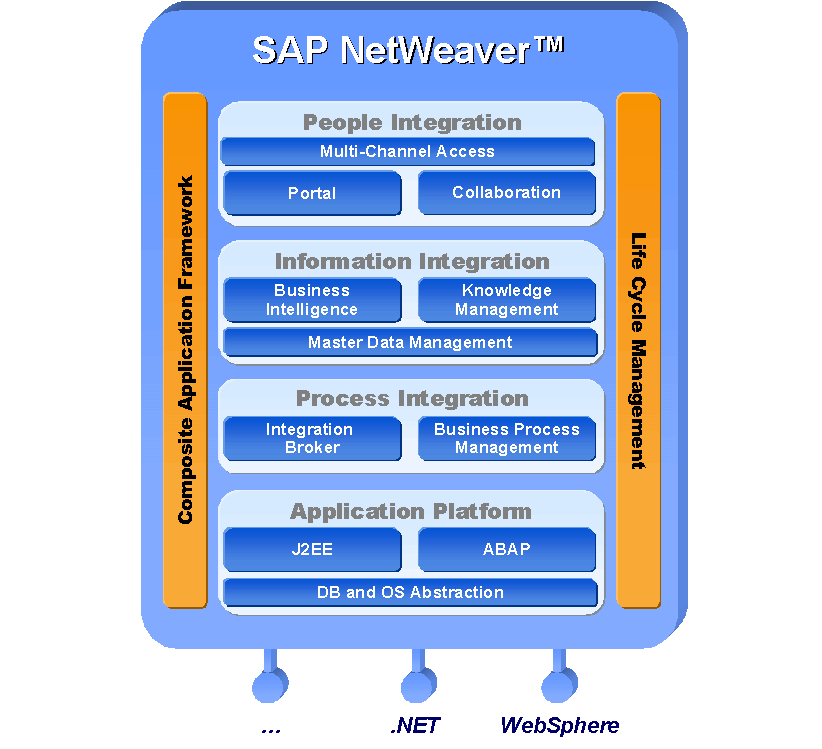
\includegraphics[width=1\linewidth]{grafiken/NetWeaver.png}
	\vspace{-20pt}
	\caption{Aufbau der \gls{sap} \gls{nw} Plattform (Quelle: \cite{NWGrundlagen})}
	\vspace{-10pt}
	\label{abb:SAPNWGrundlagen}
	\end{center}
\end{figure}

Über alle Bereiche gibt es das Life Cycle Management und das Composite Application Framework. Life Cycle Management umfasst Design, Entwicklung, Test, fortlaufender Betrieb der Applikationen und dessen Administrations- \gls{bzw} Change-Management. Daher bietet \gls{nw} Life Cycle Management für alle der Vier Bereiche an.
Das Composite Application Framework ermöglicht es, Applikationen aus verschiedenen Bereichen für \gls{nw} zu entwickeln.

%%%%%%%%%%%%%%%%%%%%%%%
%% KAPITEL Datenbank %%
%%%%%%%%%%%%%%%%%%%%%%%
%% STEFFEN
%%%%%%%%%%%%%%%%%%%%%%%
\section{Datenbanken}
Ein \gls{sap}-System stellt generell nur die Anwendungssoftware zur Verfügung. Die notwendigen Daten werden in einer (externen) \gls{db} bereitgestellt. Daher ist die Auswahl der \gls{db} genauso wichtig, wie die Auswahl der Hardware-Plattform und des Betriebssystems.
Die \gls{sap} Datenbank ist eine Ansammlung an verbundenen Tabellen, die als \gls{rdbms} bekannt ist. Manche Produkte, wie zum Beispiel \gls{erp}, bestehen aus mehr als 40.000 Tabellen \cite{SAPin24hrs}.

\subsection{SAP HANA}
\label{sec:db-hana}

\subsubsection{Einführung}
\label{sec:db-hana-intro}
% historische, hana studio, rowstore (anderer Aufbau als bei herkömml. dbs)
\gls{sap} \gls{hana} kombiniert die Funktionen einer \gls{db}, der Datenverarbeitung und die Funktionen einer Anwendungsplattform auf Ebene des Hardware Arbeitsspeichers. \gls{hana} bietet \gls{ua} Bibliotheken für Vorhersage, Planung, Textanalyse oder Geschäftsanalysen an.\\

\begin{figure}[H]
	\begin{center}
	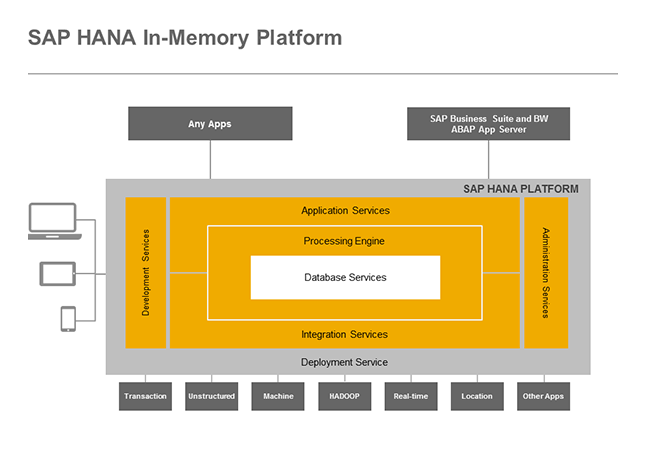
\includegraphics[width=1\linewidth]{grafiken/hana-features-overview.png}
	\vspace{-20pt}
	\caption{Aufbau der \gls{sap} \gls{hana} Plattform \cite{SAPHanaAbout}}
	\vspace{-10pt}
	\label{abb:SAPHanaAbout}
	\end{center}
\end{figure}

\gls{hana} verwendet in seiner \gls{db} einen sogenannten spalten basierten Datenspeicher, welcher im Arbeitsspeicher abgespeichert wird. Dieser Datenspeicher ist durch verschiedene Sicherheitsfeatures vor Datenverlust bei Stromausfall oder ähnlichem gesichert.
Dadurch, dass Anwendungen direkt auf der \gls{hana} Instanz ausgeführt werden können, vereinfacht es die Entwicklung von Applikationen im Umfeld von großen Datenmengen. In Abbildung \ref{abb:SAPHanaAbout} ist die Struktur von \gls{hana} abgebildet. Hier wird gezeigt, dass \gls{hana} nicht nur eine \gls{db} ist, sondern weitaus mehr.

\subsubsection{Hands On}
\label{sec:db-hana-ho}
% welche wichtigen Befehle gibt es
Für dieses Kapitel wurde eine \gls{hana} Instanz von Grund auf konfiguriert und für den Einsatz vorbereitet. 
Als Grundlage für unser Testsystem dient ein mit VMWare virtualisierter Server mit folgenden Spezifikationen
\begin{itemize}
	\item \gls{cpu} \ldots Intel(R) Xeon(R) CPU E7- 4870  @ 2.40GHz mit 10vCores
	\item \gls{ram} \ldots 127 Gigabyte
	\item \gls{hdd} \ldots 180 Gigabyte
	\item \gls{os} \ldots Suse Enterprise Linux 11.2	
\end{itemize}

Aufgrund von Komplexitäts- und Zeitgründen gehe ich an dieser Stelle nicht weiter auf die Installation der \gls{hana} Instanz ein, lediglich ist zu erwähnen, dass man gewisse Instanz Attribute zum späteren Login benötigt. Dies sind \gls{ua} \emph{Instance}, \emph{Sid} und natürlich Login Daten für den \emph{System} Benutzer.\\
Zum benutzen der \gls{hana} Instanz benötigt man das Programm "`\gls{sap} \gls{hana} Studio"'. Dieses steht unter folgendem Link\footnote{\url{http://scn.sap.com/community/developer-center/hana}} zum Download zur Verfügung.

Nachdem das System im \gls{hana} Studio (mithilfe der Instanz Attribute) hinzugefügt wurde, können alle Funktionen von \gls{hana} verwenden werden.

Zunächst befüllen wir eine Datenbank mit mehreren Tabellen, die mit Hilfe eines \gls{sql} Scripts mit Zufallsdaten gefüllt werden (siehe \ref{anhang:hanasql}). In unserem Beispiel werden 10 Millionen Datensätze eingefügt. Um zu prüfen, wie viele Datensätze eine Tabelle enthält gehen wir wie in \ref{hana:countselect} dargestellt vor.

\lstset{language=SQL, caption={Beispieldaten zählen}, label={hana:countselect}}								
\begin{lstlisting}
	SELECT count(*) FROM "SYSTEM"."TABLENAME"
\end{lstlisting}

Aufgrund der Komplexität des Scripts dauerte das Einfügen auf unserer \gls{hana} Testmaschine mehr als 40 Stunden. Dies kann je nach Hardware deutlich variieren.\\

\lstset{language=SQL, caption={Beispieldaten selektieren}, label={hana:select}}								
\begin{lstlisting}
	SELECT * FROM "SYSTEM"."TABLENAME"
\end{lstlisting}

Um alle 10 Millionen Datensätze zu selektieren (Listing \ref{hana:select}), benötigt die \gls{hana} \gls{db} lediglich weniger als 285 Millisekunden. Dies zeigt, dass auch weitaus mehr Datensätze selektiert und damit Anwendungen exponentiell im Vergleich zu herkömmlichen \gls{db} verschnellert werden können. Wie sich \gls{hana} im Vergleich mit anderen herkömmlichen \gls{db} verhält, wird in Kapitel \ref{sec:db-hana-vgl} behandelt.

\begin{center}
	\begin{verbatim}
		Statement 'SELECT * FROM "SYSTEM"."SALES_F"' 
		successfully executed in 284 ms 214 µs  
		(server processing time: 275 ms 793 µs)
	\end{verbatim}
\end{center}

\subsubsection{Vergleich}
\label{sec:db-hana-vgl}
% zeitvergleich oracle / hana db select
Zum praktischen Vergleich mit der öffentlich verfügbaren und häufig im Web-Bereich verwendeten MySQL \gls{db}, wurden Testdatensätze von MySQL\footnote{\url{https://dev.mysql.com/doc/employee/en/employees-installation.html}} in eine MySQL \gls{db} eingefügt. Eine der Tabellen aus dem Beispiel enthält \emph{2.844.047} Datensätze. Somit ist eine vergleichbare Basis geschaffen, welche man mit einfachen mathematischen Mitteln vergleichen kann. Leider ist die hießig verwendete Hardware weitaus schlechter als die verwendete Hardware für unsere \gls{hana} Testmaschine. Nichtsdestotrotz ist ein Vergleich an dieser Stelle durchaus repräsentabel, da herkömmliche Datenbanken nicht voll im Arbeitsspeicher arbeiten. Aus diesem Grund bringen an dieser Stelle größere Hardwarekomponenten nur bedingt einen Vorteil.
Mithilfe von der Programmiersprache PHP\footnote{\url{http://php.net}} selektieren (Listing \ref{anhang:mysql-select}) wir die gewünschten Datensätze aus unserer \gls{db} und zeigen uns die Dauer der Selektion an. Dabei verwenden wir die PHP Funktion \emph{microtime()}\footnote{\url{http://php.net/manual/en/function.microtime.php}} und bauen uns einen sehr genauen Timer, um die Selektion aus der MySQL \gls{db} zu messen.
MySQL benötigt also für die \emph{2.844.047} Datensätze ca. \emph{3.27} Sekunden. Somit ist die \gls{hana} \gls{db} mehr als 41 mal schneller als die MySQL \gls{db}. 

\begin{center}
	\begin{verbatim}
		Selektierte Sätze von employees.salaries: 2844047 
		Dauer: 3.2692410945892 Sekunden 
	\end{verbatim}
\end{center}

\subsection{Sonstige}
\label{sec:db-sonstige}
% welche datenbanken kann man sonst benutzen
% oracle,...
\gls{sap} unterstützt unter anderem Microsoft \gls{sql}-Server, \gls{sql} Azure, \gls{ibm} DB2 und die Oracle-Datenbank. Weiterhin unterstützt \gls{sap} natürlich seine eigenen Datenbanken MaxDB, Sybase und die zuvor behandelte \gls{hana}.